\begin{enumerate}

\item  For $p\brak{x} = x + 5$ 
\begin{flushleft}
The given equation can be represented as follows in the vector form:
\end{flushleft}
\begin{align}
\myvec{
5 & -1
}
\vec{x} + 5 = 0
\end{align}

To find the roots $y=0$: 
\begin{align}
\vec{x} &= \myvec{x_1\\0} \\
x_1 + 5 &= 0 \\
x_1 &= -5
\end{align}

%%%%%%%%%%%%%%%%%%%%
\item  For $p\brak{x} = x - 5$
\begin{flushleft}
The given equation can be represented as follows in the vector form:
\end{flushleft}
\begin{align}
\myvec{
5 & -1 
}
\vec{x} - 5 = 0
\end{align}

To find the roots $y=0$:
\begin{align}
\vec{x} &= \myvec{x_1\\0} \\
x_1 - 5 &= 0 \\
x_1 &= 5
\end{align}
%%%%%%%%%%%%%%%%%%%%
\item  For $p\brak{x} = 2x + 5$
\begin{flushleft}
The given equation can be represented as follows in the vector form:
\end{flushleft}
\begin{align}
\myvec{
2 & -1 
}
\vec{x} + 5 = 0
\end{align}

To find the roots $y=0$:
\begin{align}
\vec{x} &= \myvec{x_1\\0} \\
2x_1 + 5 &= 0 \\
x_1 &= \frac{-5}{2}
\end{align}
%%%%%%%%%%%%%%%%%%%%
\item  For $p\brak{x} = 3x - 2$
\begin{flushleft}
The given equation can be represented as follows in the vector form:
\end{flushleft}
\begin{align}
\myvec{
3 & -1 
}
\vec{x} - 2 = 0
\end{align}

To find the roots $y=0$:
\begin{align}
\vec{x} &= \myvec{x_1\\0} \\
3x_1 - 2 &= 0 \\
x_1 &= \frac{2}{3}
\end{align}
%%%%%%%%%%%%%%%%%%%%
\item 
 For $p\brak{x} = 3x$
\begin{flushleft}
The given equation can be represented as follows in the vector form:
\end{flushleft}
\begin{align}
\myvec{
3 & -1 
}
\vec{x}  = 0
\end{align}

To find the roots $y=0$:
\begin{align}
\vec{x} &= \myvec{x_1\\0} \\
3x_1  &= 0 \\
x_1 &= 0
\end{align}
\begin{figure}[!ht] 
\centering
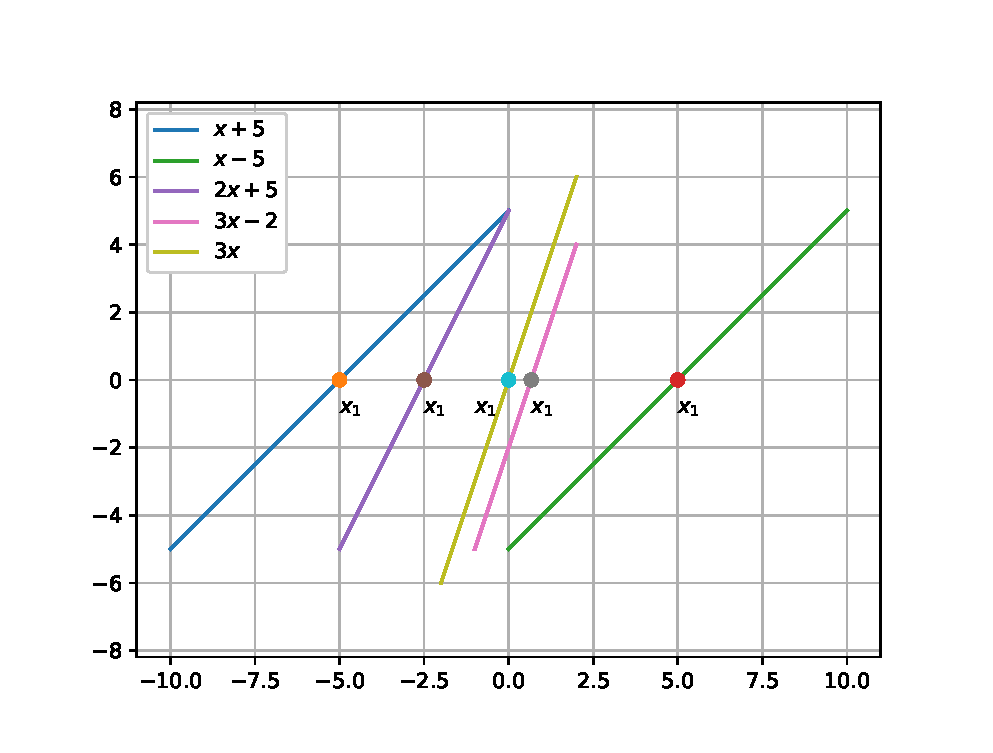
\includegraphics[width=\columnwidth]{./solutions/2/figs/line_ex/lines_and_planes/final_eq.eps}
\caption{}
\label{fig:3.7.2_eq_lines_and_planes}
\end{figure}
 
The  following Python code generates Fig \ref{fig:3.7.2_eq_lines_and_planes}
\begin{lstlisting}
solutions/2/codes/line_ex/lines_and_planes/linear_eq_roots.py
\end{lstlisting}

\end{enumerate}
